\section*{CHƯƠNG 3. THIẾT KẾ HỆ THỐNG}
    \addcontentsline{toc}{section}{\numberline{}CHƯƠNG 3. PHƯƠNG PHÁP LUẬN}
    
\setcounter{section}{3}
    \setcounter{subsection}{0}
        \setcounter{figure}{0}
            \setcounter{table}{0}
%%-------------------------------------------------------%%
% --------------------------------------------------------%
%---------------------------------------------------------%

\subsection{Phân tích yêu cầu hệ thống}


\begin{figure}[!ht]
    \centering
    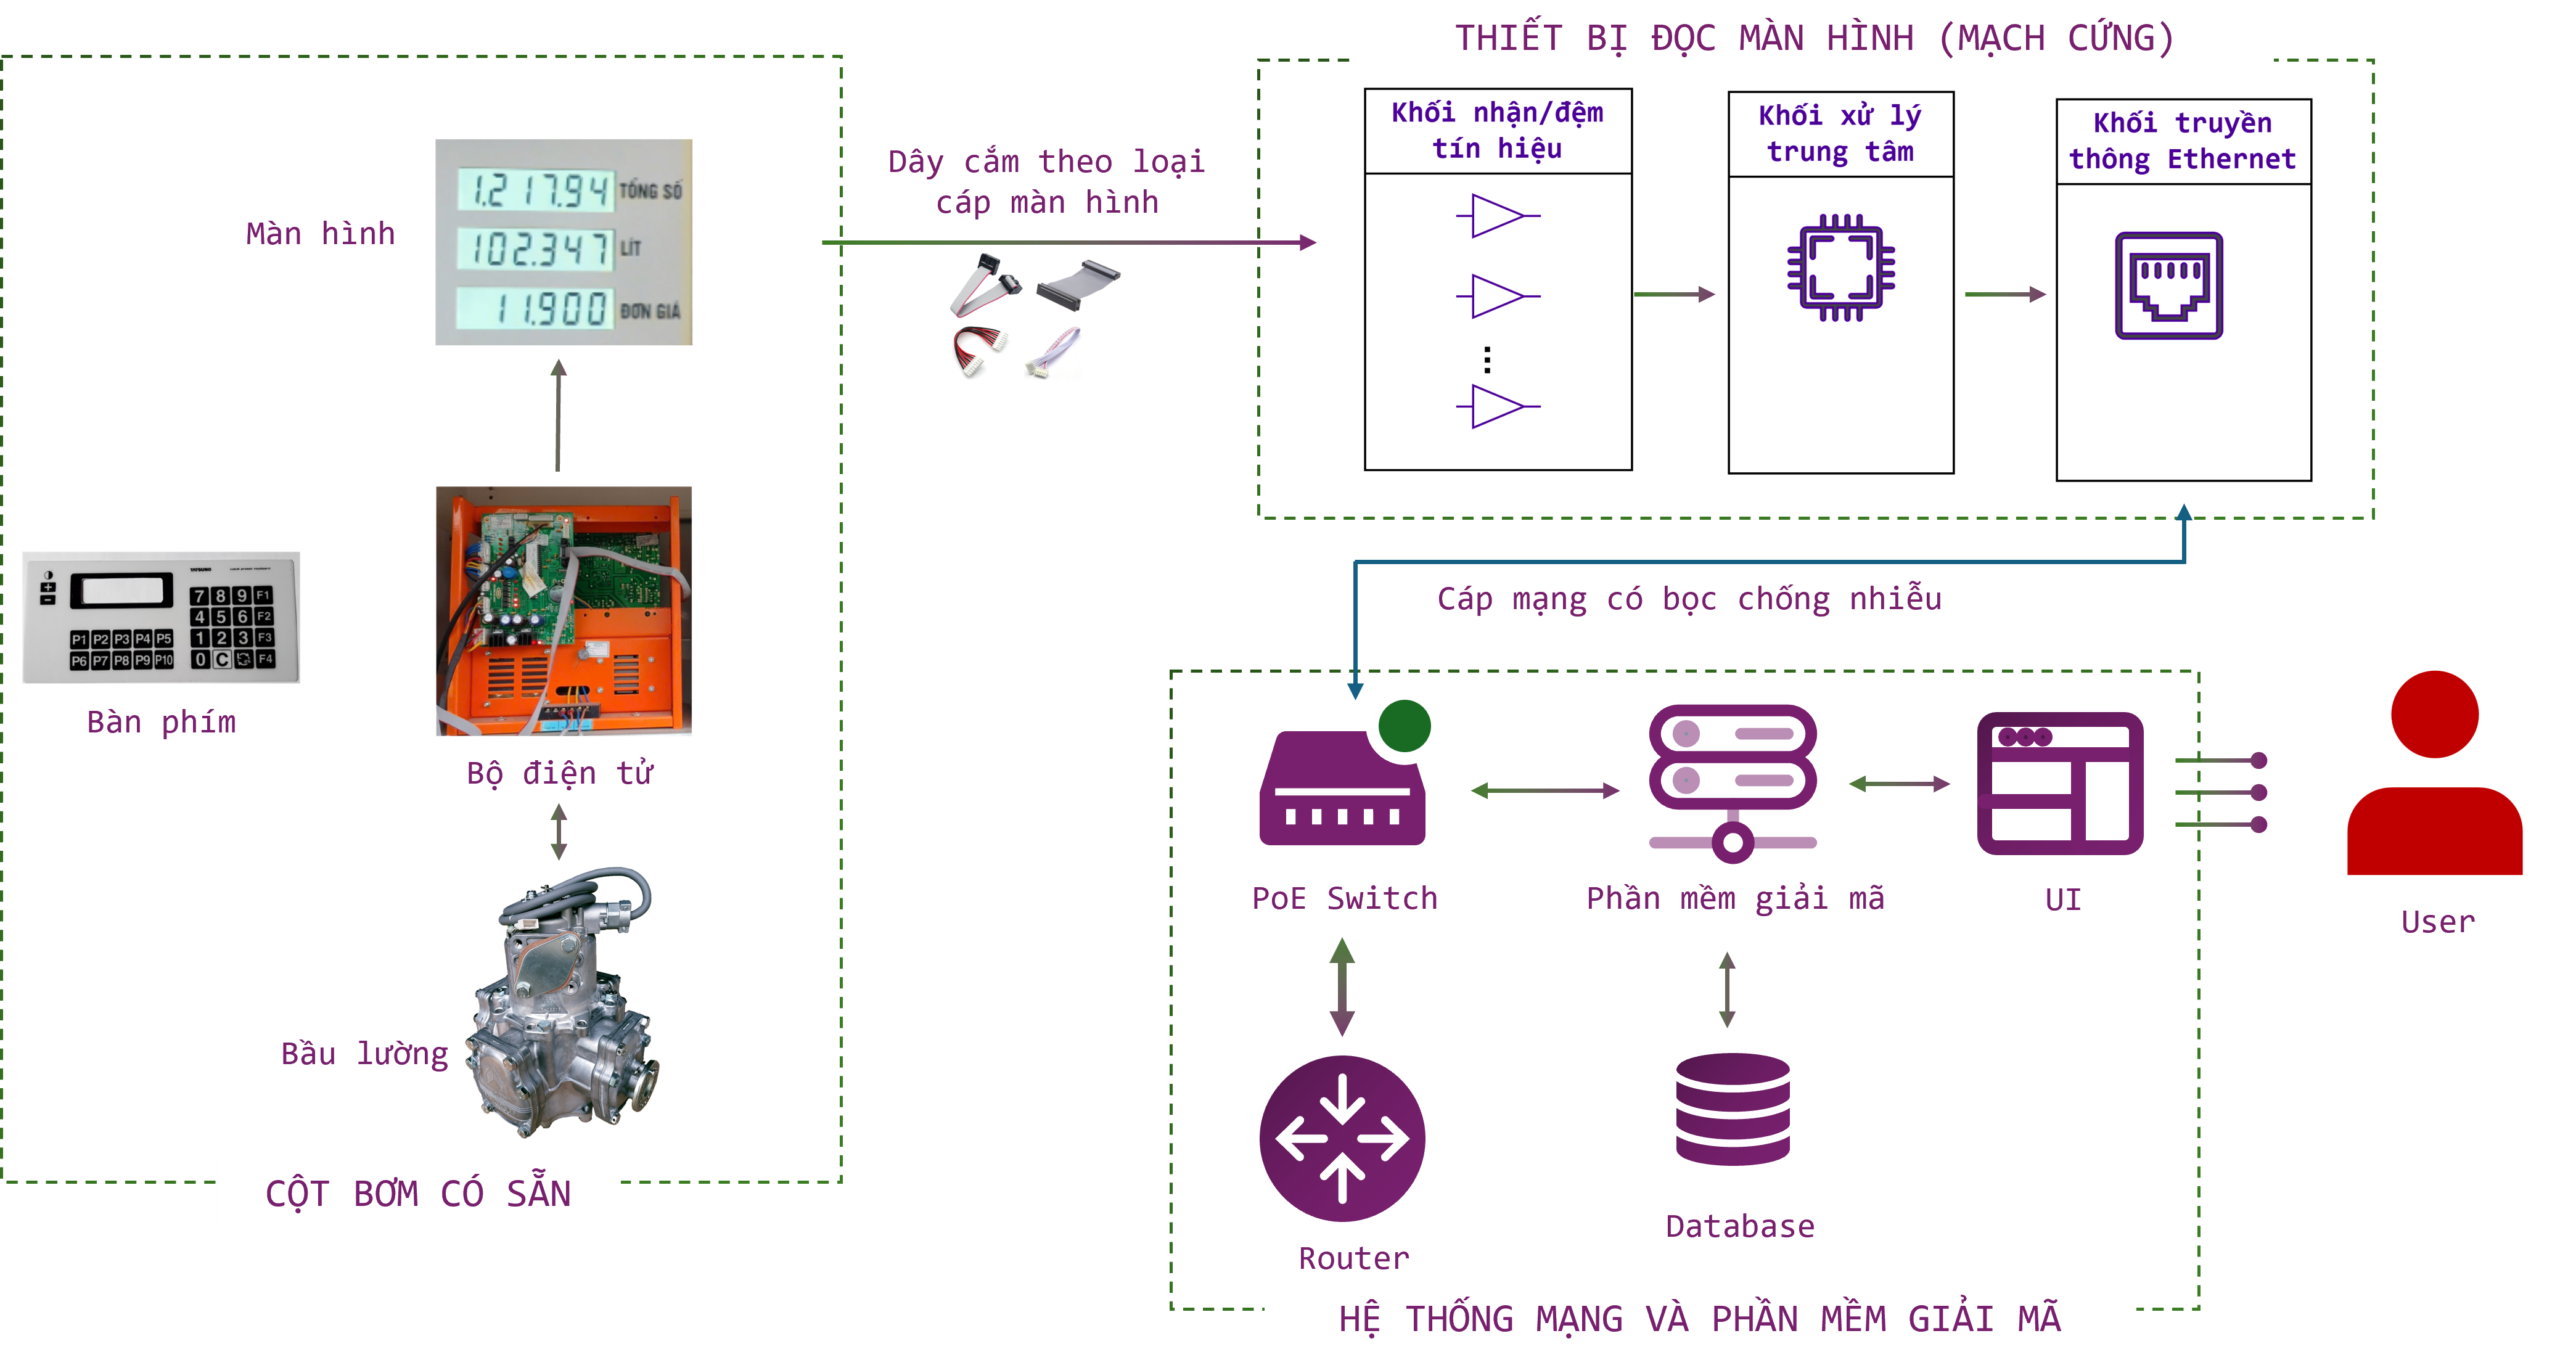
\includegraphics[width=1.0\linewidth]{Figures/Chap3_FunctionBlock-implementation.png}
    \caption{Các thành phần của hệ thống}
    \label{fig:hinh3.1}
\end{figure}

Các thành phần chính của hệ thống bao gồm:

\subsubsection{Thiết bị đọc ghi màn hình}


\hspace{0.8cm} Là mạch cứng gắn vào màn hình cột bơm, thu dữ liệu thô màn hình:
\begin{itemize}
   
    \item Kích cỡ: vừa, có thể lắp đặt trong cột bơm
    \item Tần số lấy mẫu: 100Hz
    \item Cấp nguồn riêng
    \item Nguồn và tín hiệu vào được cách ly quang, đảm bảo không có tín hiệu quay ngược trở lại màn hình
    \item Có 2 relay đóng ngắt có thể nối nối tiếp với cột bơm
    \item Giao tiếp, gửi dữ liệu thông qua Ethernet
    \item (Optional) Đầu vào tín hiệu (cáp và bộ chuyển đổi tín hiệu) có thể thích hợp với nhiều loại màn hình khác ngoài ZCheng để phục vụ thu thập và phân tích thêm các loại cột bơm khác.
    
\end{itemize}



\subsubsection{Phần mềm giải mã}

\hspace{0.8cm} Phần mềm giải mã đặt trong máy tính nội bộ tại trạm:

\begin{itemize}
    \item Đọc và giải mã tín hiệu tới màn hình với tần số 100Hz.
    \item Giao diện phần mềm hiển thị màn hình đã giải mã theo thời gian thực
    \item Phát hiện, lưu trữ các phiên bơm. Giao diện hiển thị các phiên bơm đã lưu trữ.
    \item Điều khiển đóng ngắt relay.
    \item Có cơ chế cập nhật firmware (OTA) cho thiết bị.    
\end{itemize}

\subsubsection{Hệ thống mạng}

\begin{itemize}
    \item POE Switch cấp nguồn riêng cho thiết bị đọc ghi màn hình
    \item Router điều khiển mạng LAN, cấp phát IP cho thiết bị
    \item Các thiết bị (thiết bị đọc ghi màn hình và phần mềm giải mã trong máy tính nội bộ) có thể tự động dò tìm và kết nối với nhau.
\end{itemize}

\subsection{Mô hình thiết kế tổng thể}

\hspace{0.8cm} Phần này nêu ra sơ đồ khối chức năng các thành phần hệ thống. Qua đó mô tả chức năng cụ thể của thành phần thông qua các khối, đồng thời mô tả cách các khối giao tiếp với nhau.

\subsubsection{Sơ đồ khối chức năng thiết bị đọc ghi màn hình (Device)}

\begin{figure}[!ht]
    \centering
    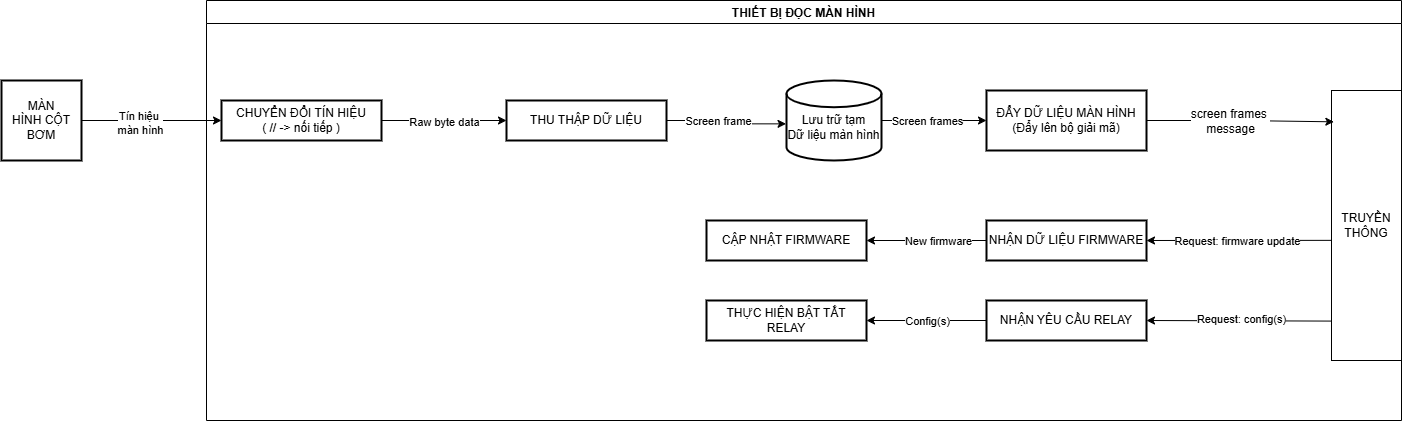
\includegraphics[width=1.0\linewidth]{Figures/Chap3_Device-FunctionBlock.png}
    \caption{Sơ đồ khối chức năng thiết bị đọc ghi màn hình (Device)}
    \label{fig:hinh3.2}
\end{figure}

\textbf{Giải thích các khối chức năng:} 

\begin{itemize}
    \item \textbf{Chuyển đối tín hiệu: }
    \subitem Nếu tín hiệu gửi tới màn hình cột bơm là nối tiếp, khối này đệm tín hiệu nối tiếp tới bộ Thu thập dữ liệu
    \subitem Nếu tín hiệu gửi tới màn hình cột bơm là song song, có nhiều chân dữ liệu, khối này chuyển đổi tín hiệu từ các chân thành tín hiệu nối tiếp -> chuyển đổi thành các SPI frame để đệm tới bộ Thu thập dữ liệu.
    \item \textbf{Thu thập dữ liệu: } Thu thập các byte data tổng hợp thành các screen frame, lưu tạm vào 1 in-mem database.
    \item \textbf{Đẩy dữ liệu lên màn hình: } Thiết bị đọc màn hình tạo 1 message (request message) gồm nhiều screen frame để đẩy lên máy tính local
    \item \textbf{Nhận và cập nhật firmware mới: } Thiết bị đọc màn hình có thể nhận firmware mới từ máy tính local hoặc Logi Service và tự động cập nhật, khởi động lại
    \item \textbf{Nhận và cập nhật relay:} Thiết bị đọc ghi màn hình có thể nhận và thực hiện yêu cầu bật tắt relay 
    \item \textbf{Truyền thông:} Lấy địa chỉ IP, dò tìm địa chỉ của phần mềm giải mã và tự động kết nối. Truyền nhận dữ liệu với phần mềm giải mã thông qua mạng LAN.

\end{itemize}

\subsubsection{Sơ đồ khối chức năng phần mềm giải mã (Device Service)}

\begin{figure}[!ht]
    \centering
    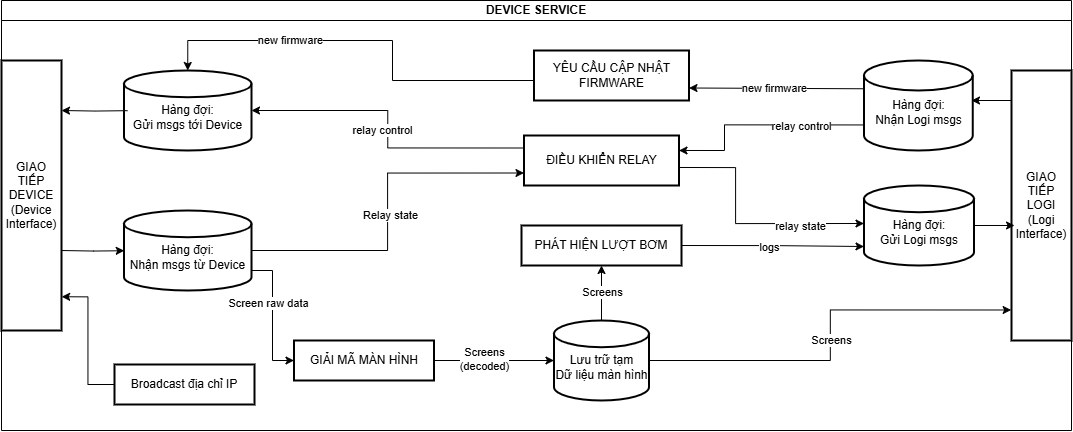
\includegraphics[width=1.0\linewidth]{Figures/Chap3_DeviceService-function-block.png}
    \caption{Sơ đồ khối chức năng phần mềm giải mã và chốt phiên bơm (Device Service)}
    \label{fig:hinh3.3}
\end{figure}

\textbf{Giải thích các khối chức năng:}

\begin{itemize}
    \item \textbf{Giao tiếp với Device (Thiết bị đọc ghi màn hình):} 
    \subitem Khối này được thiết kế chạy trên 1 luồng độc lập, nghe các yêu cầu kết nối từ thiết bị đọc ghi màn hình, kiểm tra và giữ kết nối nếu thiết bị hợp lệ 
    \subitem Truyền nhận gói tin với thiết bị đọc ghi và đẩy dữ liệu tới các khối khác để xử lý logic chính.

    \item \textbf{Giao tiếp với giao diện (GUI App):} Giữ kết nối và truyền nhận dữ liệu với phần mềm giao diện bao gồm:
    \subitem Stream dữ liệu màn hình đã giải mã theo thời gian thực.
    \subitem Gửi các phiên bơm (log) phát hiện được và trạng thái relay.
    \subitem Nhận các yêu cầu từ giao diện: cập nhật firmware, relay.
    \item \textbf{Giải mã màn hình và phát hiện phiên bơm:} Giải mã các gói tin dạng byte theo từng loại màn hình để được dữ liệu màn hình thời gian thực (số tiền, lít, đơn giá). Từ đó phát hiện trạng thái của máy (đang dừng và dừng trong bao nhiêu giây, đang tăng, reset) và phát hiện phiên bơm.
    \item \textbf{Cập nhật firmware:} Nhận file firmware từ giao diện, kiểm tra và thực hiện OTA với thiết bị đọc màn hình 
    \item \textbf{Điều khiển relay:} Chuyển tiếp gói tin yêu cầu bật tắt relay tới thiết bị đọc ghi màn hình
\end{itemize}


\subsection{Thiết kế phần cứng thiết bị đọc màn hình}

\subsubsection{Sơ đồ khối phần cứng thiết bị đọc màn hình}


\begin{figure}[!ht]
    \centering
    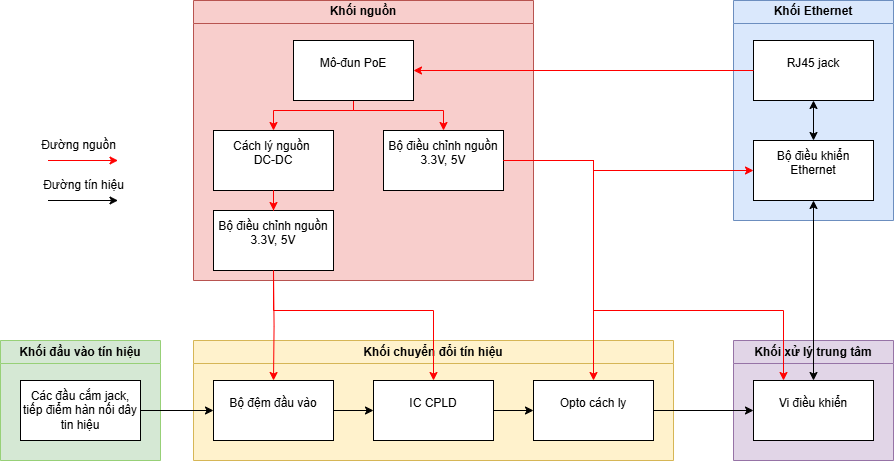
\includegraphics[width=1.0\linewidth]{Figures/Chap3_Device-Hardware-implementation-function-block.png}
    \caption{Sơ đồ khối triển khai phần cứng thiết bị đọc ghi màn hình}
    \label{fig:hinh3.4}
\end{figure}

Thiết bị mạch cứng được cấp nguồn riêng bởi POE Switch. Nguồn và tín hiệu vào được các ly bởi bộ cách ly nguồn DC-DC, các bộ đệm đầu vào và Opto cách ly, đảm bảo không ảnh hưởng tới nguồn cấp của cột bơm cũng như không có tín hiệu hay nhiễu đẩy ngược về cột bơm.

Khối đầu vào tín hiệu và khối chuyển đổi tín hiệu cũng được thiết kế thêm để thu và khảo sát được nhiều loại màn hình khác, phục vụ cho việc mở rộng chức năng hệ thống.

Thiết bị giao tiếp với phần mềm giải mã thông qua mạng LAN, sử dụng khối Ethernet.

\subsubsection{Lựa chọn linh kiện}

\textbf{a.  Khối xử lý trung tâm}

 Yêu cầu lựa chọn:
\begin{itemize}
    \item Có 2 cổng giao tiếp SPI: mục đích để giao tiếp với khối chuyển đổi tín hiệu và với khối Ethernet. 
    \item Bộ nhớ flash lớn hơn 220KB (chứa được 2 firmware, mỗi firm ~ 110kB)
\end{itemize}

Từ những yêu cầu trên , lựa chọn STM32F407VET6 là vi điều khiển xử lý trung tâm. Các tính năng nổi bật của STM32F407VET6:

\begin{itemize}
    \item Vi điều khiển sử dụng lõi ARM Cortex-M4 32-bit, tốc độ tối đa 168 MHz, tích hợp bộ xử lý dấu chấm động (FPU) và tập lệnh DSP, phù hợp cho các ứng dụng điều khiển và xử lý tín hiệu thời gian thực.
    
    \item Bộ nhớ Flash Main Memory 512 KB, được chia thành các sector như sau:  
    
    \begin{itemize}
        \item Sector 0-3: mỗi sector 16 KB  
        \item Sector 4: 64 KB  
        \item Sector 5, 6 và 11: mỗi sector 128-KB  
    \end{itemize}

    \item Cho phép linh hoạt khi lưu nhiều firmware (ví dụ dual-bank firmware upgrade), hoặc phân vùng cho bootloader, data log, cấu hình...

    \item Tích hợp 3 cổng SPI (SPI1, SPI2, SPI3), hỗ trợ chế độ master/slave, tốc độ tối đa đến 42 MHz (SPI1) và 21 MHz (SPI2/SPI3). Phù hợp cho các giao tiếp tốc độ cao như ADC ngoại vi và module Ethernet SPI.

    \item Có tổng cộng 17 bộ Timer, gồm 12 timer 16-bit và 2 timer 32-bit. Hỗ trợ nhiều chế độ: PWM, encoder, input capture, output compare, rất hữu ích trong điều khiển động cơ, đo thời gian hoặc phát xung.

    \item Hỗ trợ nhiều chuẩn giao tiếp ngoại vi: UART, I2C, USB OTG, CAN, SDIO, Ethernet MAC - thuận tiện cho mở rộng và kết nối các module chức năng khác.

    \item Hoạt động với điện áp 1.8 V đến 3.6 V, hỗ trợ các chế độ tiết kiệm năng lượng như Sleep, Stop, và Standby - phù hợp cho ứng dụng nhúng có yêu cầu tiêu thụ điện thấp.
\end{itemize}


\begin{figure}[!ht]
    \centering
    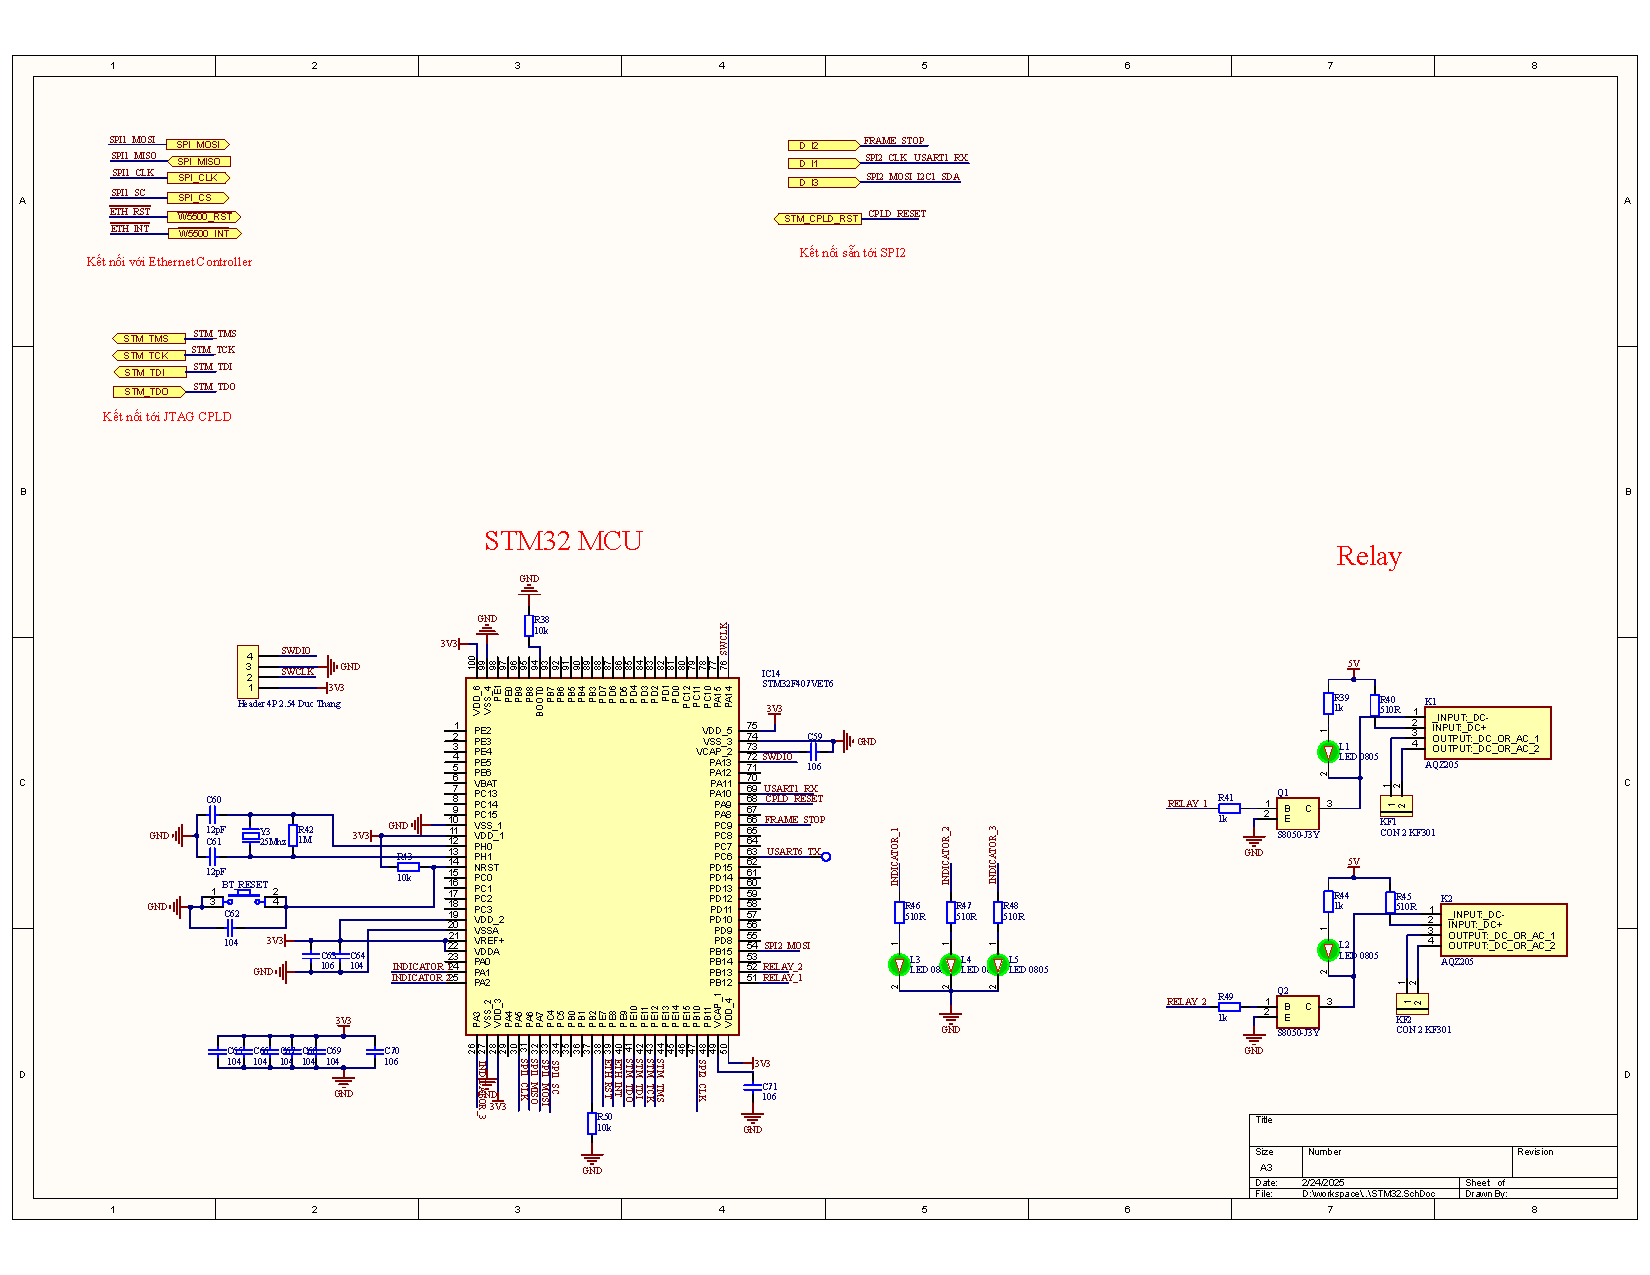
\includegraphics[width=1.0\linewidth]{Figures/Chap3_STM32-principle.pdf}
    \caption{Sơ đồ nguyên lý khối xử lý trung tâm}
    \label{fig:hinh3.5}
\end{figure}


\hspace{0.8cm} Sơ đồ nguyên lý mạch:

\begin{itemize}
    \item Nguồn cấp 3.3V được đưa vào các chân VDD và Vref của module, các chân VSS được nối đất. Thiết kế nguồn nối với đất qua các tụ Bypass có nhiệm vụ lọc nhiễu cao tần cho nguồn nuôi vi điều khiển.
    \item Sử dụng SPI1 để giao tiếp với chip Ethernet. SPI2 để giao tiếp với khối chuyển đổi dữ liệu
    \item Các chân PA1, PA2, PA3 điều khiển đèn báo led 
    \item Reset STM32 được thực hiện khi chân NRST hạ xuống mức 0:
    \begin{itemize}
        \item Điện trở kéo lên 10K$\Omega$
        \item Tụ điện: C = 100nF, giúp tạo xung reset ngắn nhưng đủ để tái khởi STM32
    \end{itemize}
    \item Mạch nạp cho STM32:
    \begin{itemize}
        \item Thiết kế mạch nạp theo chuẩn SWD
        \item Hỗ trợ nạp thông qua mạch nạp STLink
    \end{itemize}

\end{itemize}

\textbf{Khối đầu vào tín hiệu}


 Yêu cầu lựa chọn: 

Ngoài việc thu và giải mã loại màn hình ZCheng, khối đầu vào tín hiệu còn cần hỗ trợ các loại đầu vào cho màn hình khác để thu mẫu dữ liệu, phục vụ cho việc giải mã, mở rộng hệ thống sau này. Các loại đầu vào màn hình đã khảo sát được bao gồm:

\begin{itemize}
    \item Đầu vào SPI (cho màn hình ZCheng, đã giải mã được). Loại cáp: 8P 3.96mm. Số chân tín hiệu: 3
    \item Loại cáp: 5P 3.96mm, số chân tín hiệu: 2
    \item Loại cáp: IDE 10. Số chân tín hiệu 3
    \item Loại cáp: IDE 40. Số chân tín hiệu 30
\end{itemize}

Với danh sách loại đầu vào ở trên, thiết kế khối đầu vào tín hiệu gồm các đầu jack cắm và tiếp điểm hàn để đấu nối dây điên. Khối gồm 2 phần: 

\begin{itemize}
    \item Các đầu cắm cáp: hỗ trợ các loại cáp đã khảo sát.
    \item Các điểm hàn nối dây: Trường hợp các loại màn hình khác, sẽ hàn các đường tín hiệu đó thông qua các đầu tiếp điểm hàn, kèm dây điện nối (nếu cần). Vị trí mối hàn, đấu dây sẽ cố định theo từng loại tín hiệu màn hình.
\end{itemize}

Số chân tối đa cho khối đầu vào tín hiệu là 40 chân.

\begin{figure}[!ht]
    \centering
    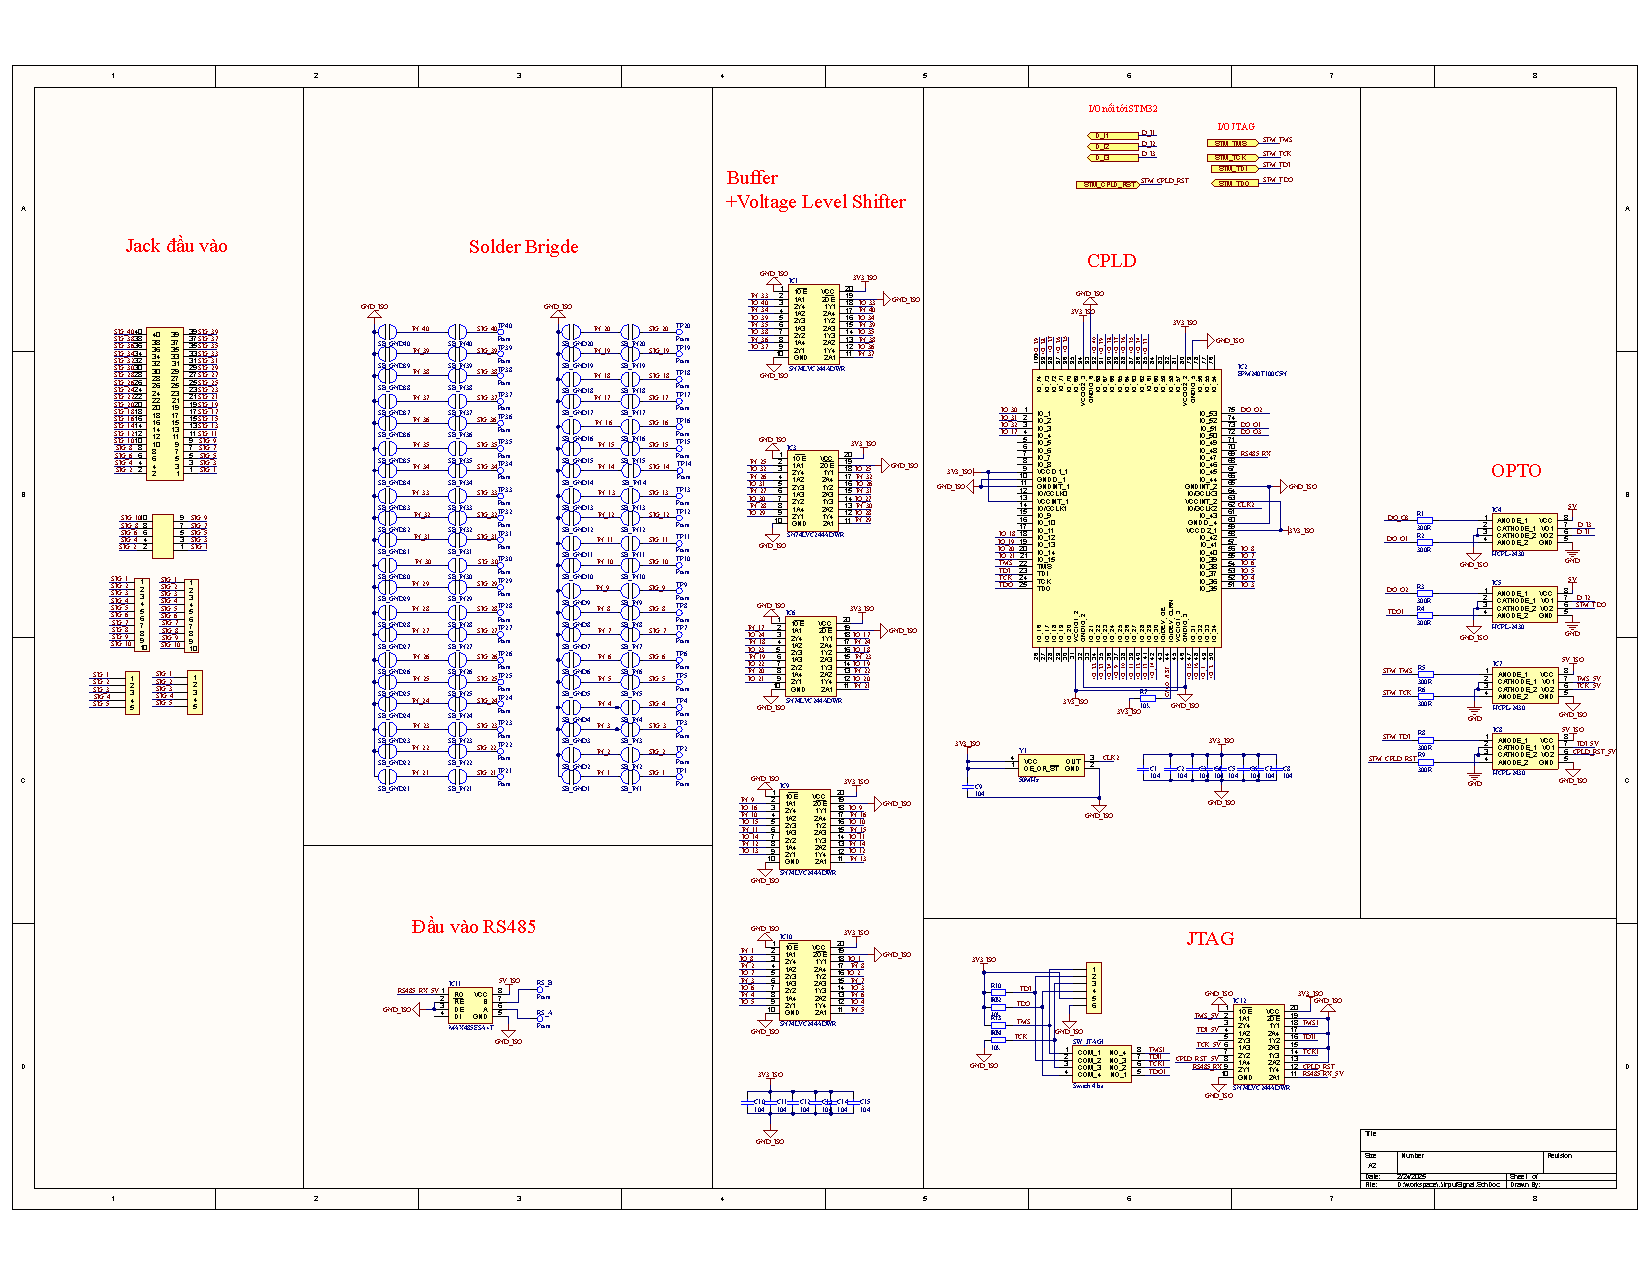
\includegraphics[width=1.0\linewidth]{Figures/Chap3_Input-signal-block-principle.pdf}
    \caption{Sơ đồ nguyên lý khối đầu vào tín hiệu}
    \label{fig:hinh3.6}
\end{figure}






















